% --------------------------------------------------------------
% This is all preamble stuff that you don't have to worry about.
% Head down to where it says "Start here"
% --------------------------------------------------------------

\documentclass[12pt]{article}

\usepackage[margin=1in]{geometry}
\usepackage{amsmath,amsthm,amssymb}
\usepackage{graphicx} %This allows to include eps figures
\usepackage{subcaption}
\usepackage[section]{placeins}
\usepackage{layout}
\usepackage{etoolbox}
% This is to include code
\usepackage{listings}
\usepackage{xcolor}
\definecolor{dkgreen}{rgb}{0,0.6,0}
\definecolor{gray}{rgb}{0.5,0.5,0.5}
\definecolor{mauve}{rgb}{0.58,0,0.82}
\lstdefinestyle{Python}{
    language        = Python,
    basicstyle      = \ttfamily,
    keywordstyle    = \color{blue},
    keywordstyle    = [2] \color{teal}, % just to check that it works
    stringstyle     = \color{green},
    commentstyle    = \color{red}\ttfamily
}

\newcommand{\N}{\mathbb{N}}
\newcommand{\Z}{\mathbb{Z}}

\newenvironment{theorem}[2][Theorem]{\begin{trivlist}
\item[\hskip \labelsep {\bfseries #1}\hskip \labelsep {\bfseries #2.}]}{\end{trivlist}}
\newenvironment{lemma}[2][Lemma]{\begin{trivlist}
\item[\hskip \labelsep {\bfseries #1}\hskip \labelsep {\bfseries #2.}]}{\end{trivlist}}
\newenvironment{exercise}[2][Exercise]{\begin{trivlist}
\item[\hskip \labelsep {\bfseries #1}\hskip \labelsep {\bfseries #2.}]}{\end{trivlist}}
\newenvironment{reflection}[2][Reflection]{\begin{trivlist}
\item[\hskip \labelsep {\bfseries #1}\hskip \labelsep {\bfseries #2.}]}{\end{trivlist}}
\newenvironment{proposition}[2][Proposition]{\begin{trivlist}
\item[\hskip \labelsep {\bfseries #1}\hskip \labelsep {\bfseries #2.}]}{\end{trivlist}}
\newenvironment{corollary}[2][Corollary]{\begin{trivlist}
\item[\hskip \labelsep {\bfseries #1}\hskip \labelsep {\bfseries #2.}]}{\end{trivlist}}

\begin{document}

% --------------------------------------------------------------
%                         Start here
% --------------------------------------------------------------

%\renewcommand{\qedsymbol}{\filledbox}

\title{Assignment 1}%replace X with the appropriate number
\author{Nalet Meinen\\ %replace with your name
Finite Element Analysis I
}

\maketitle

\section{Theory}

\begin{equation}\label{eq:1}
y(L) = \frac{FL^{2}}{6EI}(3L-L)
\end{equation}
With equation \ref{eq:1} we have the possibility to calculate the maximal displacment from beam theory.
Using thouse values provided in the assignment

$L = 300mm, F = 50N, E = 90e6 \frac{N}{mm^{2}}, I = \frac{b\cdot h^{3}}{12} = \frac{5\cdot 10^{3}}{12} =  416,67mm^{4} $ 

we come to the result in \ref{eq:2}
\begin{equation}\label{eq:2}
y(300) = \frac{50 \cdot 300^{2}}{6\cdot 90e6 \cdot 416,67}(3\cdot300-300) = 12mm
\end{equation}
\pagebreak
\section{Abaqus}

\subsection{2 x 12 elments}

\subsubsection{CPS4}
\begin{figure}[!htb]
  \centering
  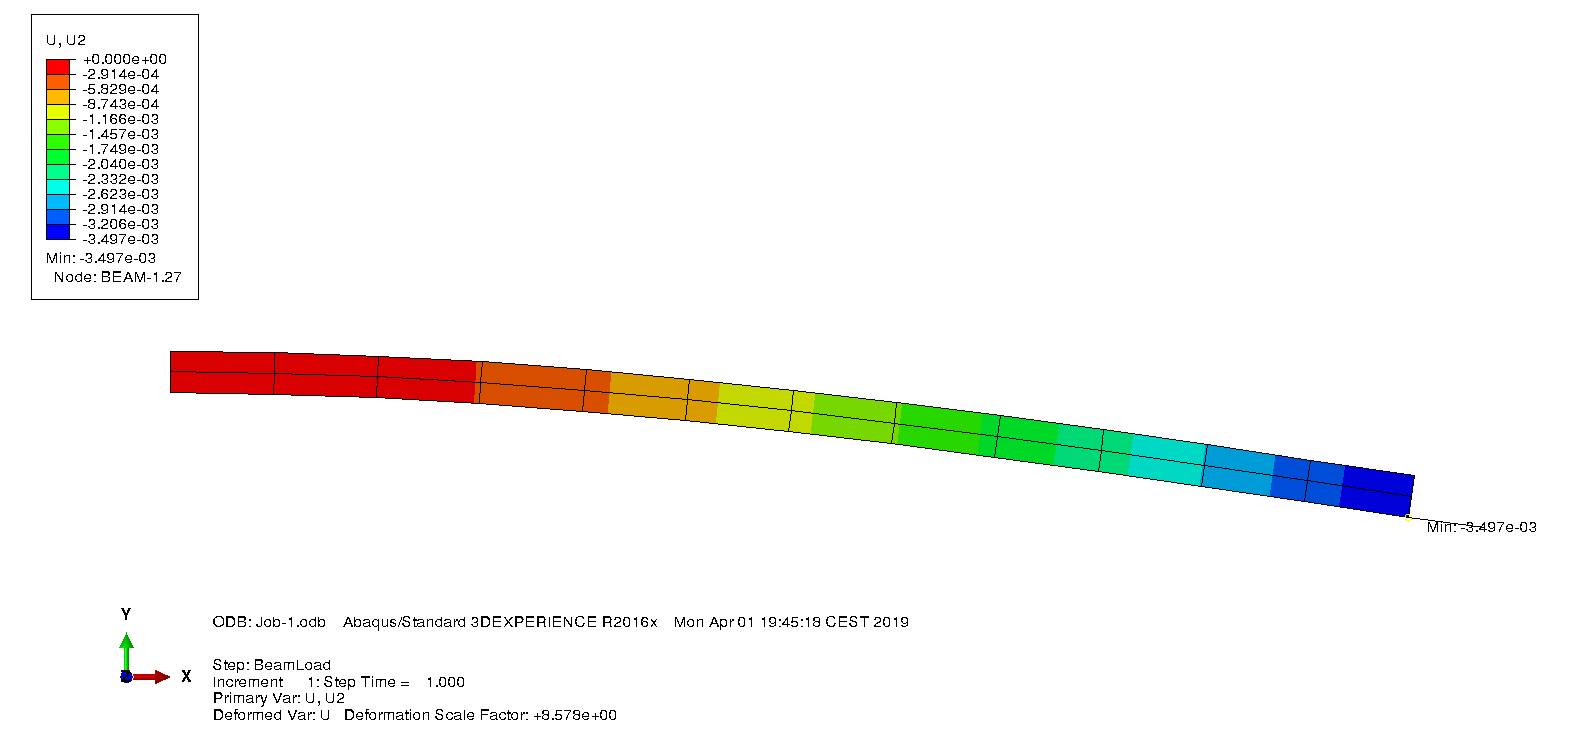
\includegraphics[width=0.8\textwidth]{pics/2_12_CPS4}
  \caption{maximal displacment: -3.50 mm}
\end{figure}
\FloatBarrier
\subsubsection{CPS8}
\begin{figure}[!htb]
  \centering
  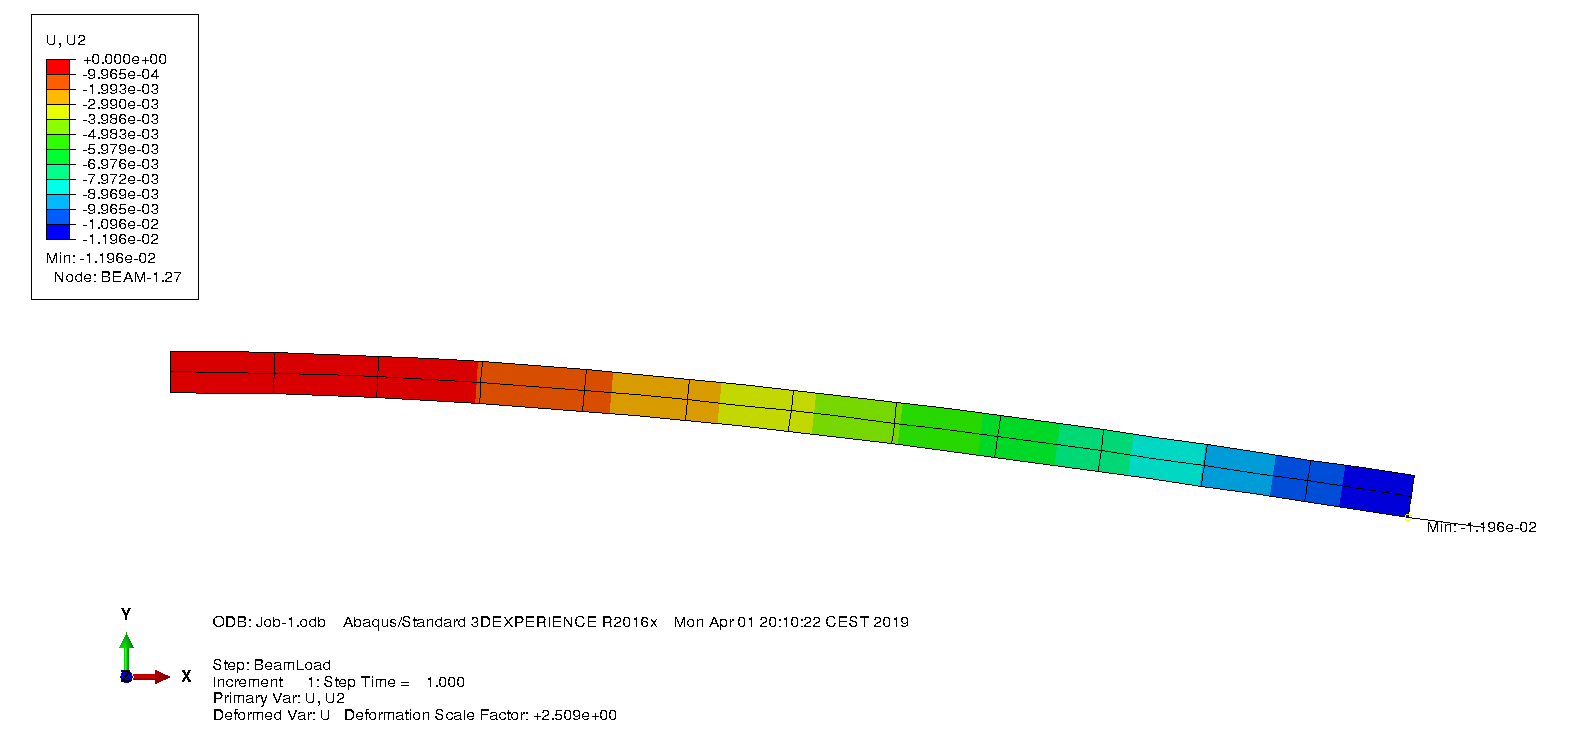
\includegraphics[width=0.8\textwidth]{pics/2_12_CPS8}
  \caption{maximal displacment: -11.96 mm}
\end{figure}
\FloatBarrier
\pagebreak
\subsubsection{CPS4R}
\begin{figure}[!htb]
  \centering
  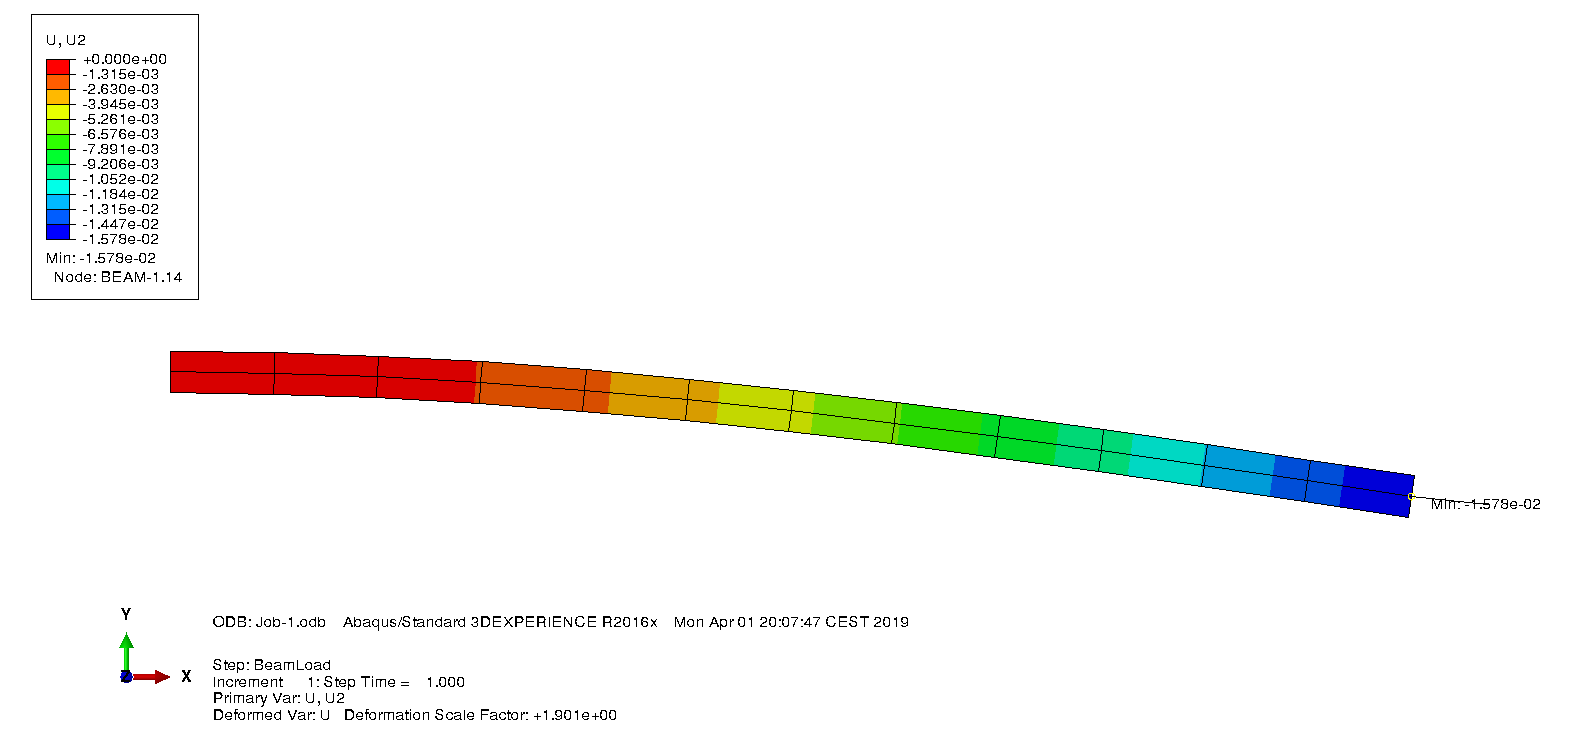
\includegraphics[width=0.8\textwidth]{pics/2_12_CPS4R}
  \caption{maximal displacment: -15.78 mm}
\end{figure}
\FloatBarrier
\subsubsection{CPS8R}
\begin{figure}[!htb]
  \centering
  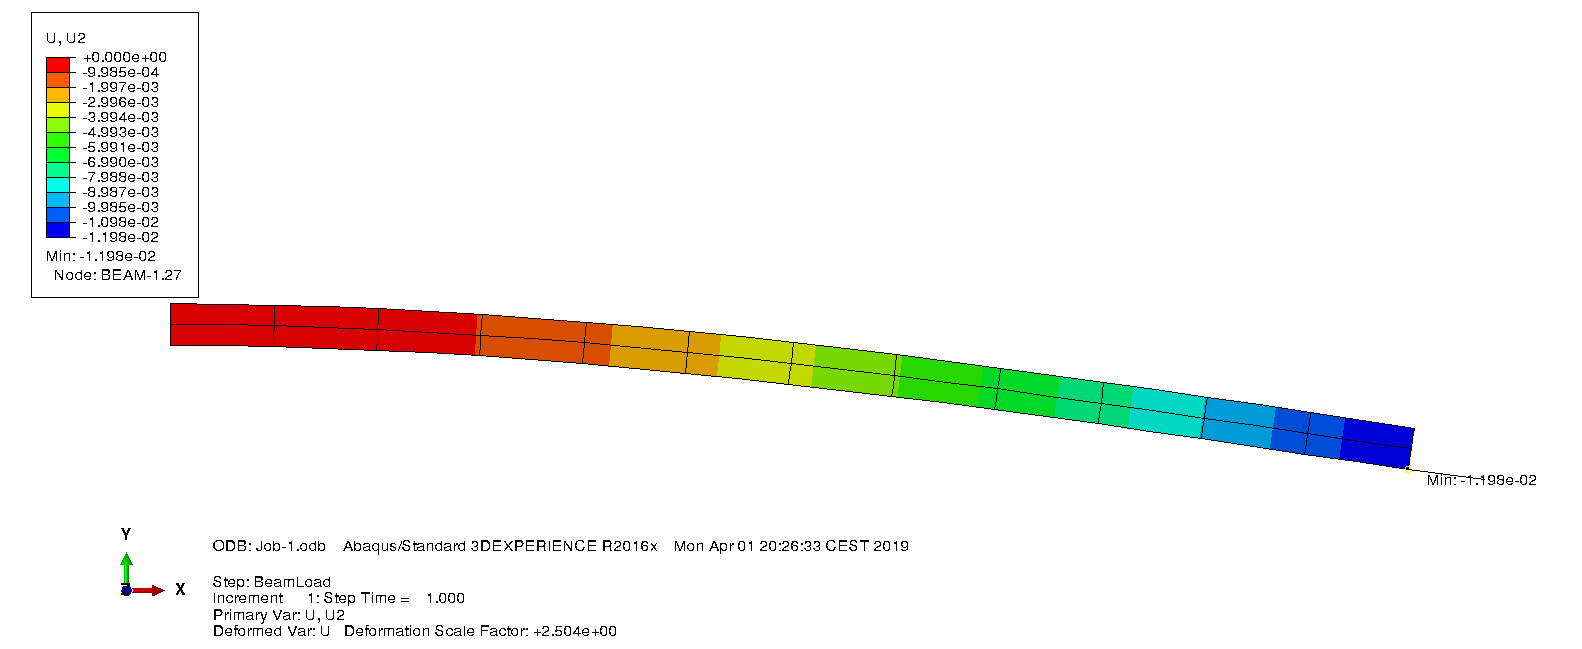
\includegraphics[width=0.8\textwidth]{pics/2_12_CPS8R}
  \caption{maximal displacment: -11.98 mm}
\end{figure}
\FloatBarrier
\pagebreak
\subsection{4 x 24 elments}

\subsubsection{CPS4}
\begin{figure}[!htb]
  \centering
  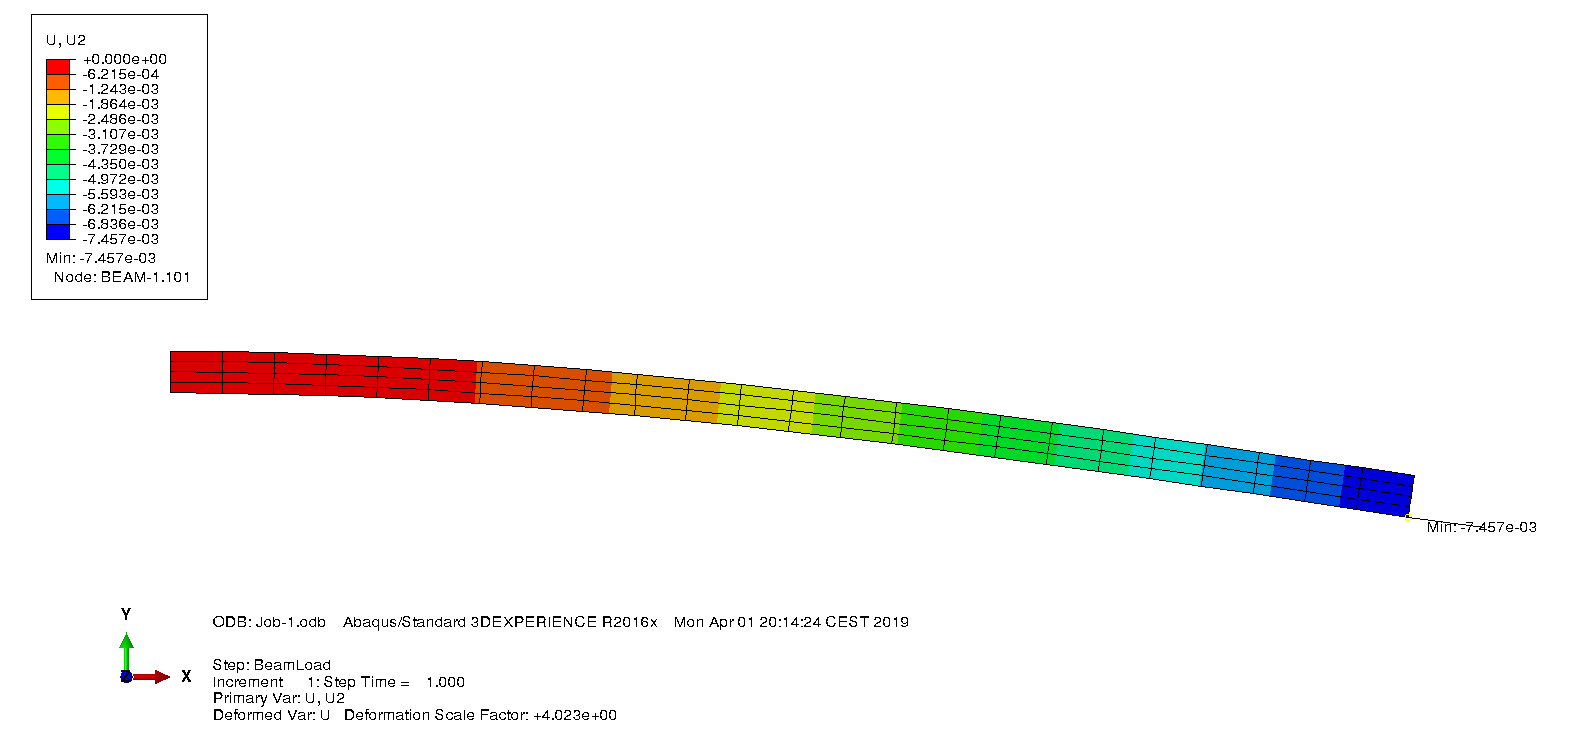
\includegraphics[width=0.8\textwidth]{pics/4_24_CPS4}
  \caption{maximal displacment: -7.46 mm}
\end{figure}
\FloatBarrier
\subsubsection{CPS8}
\begin{figure}[!htb]
  \centering
  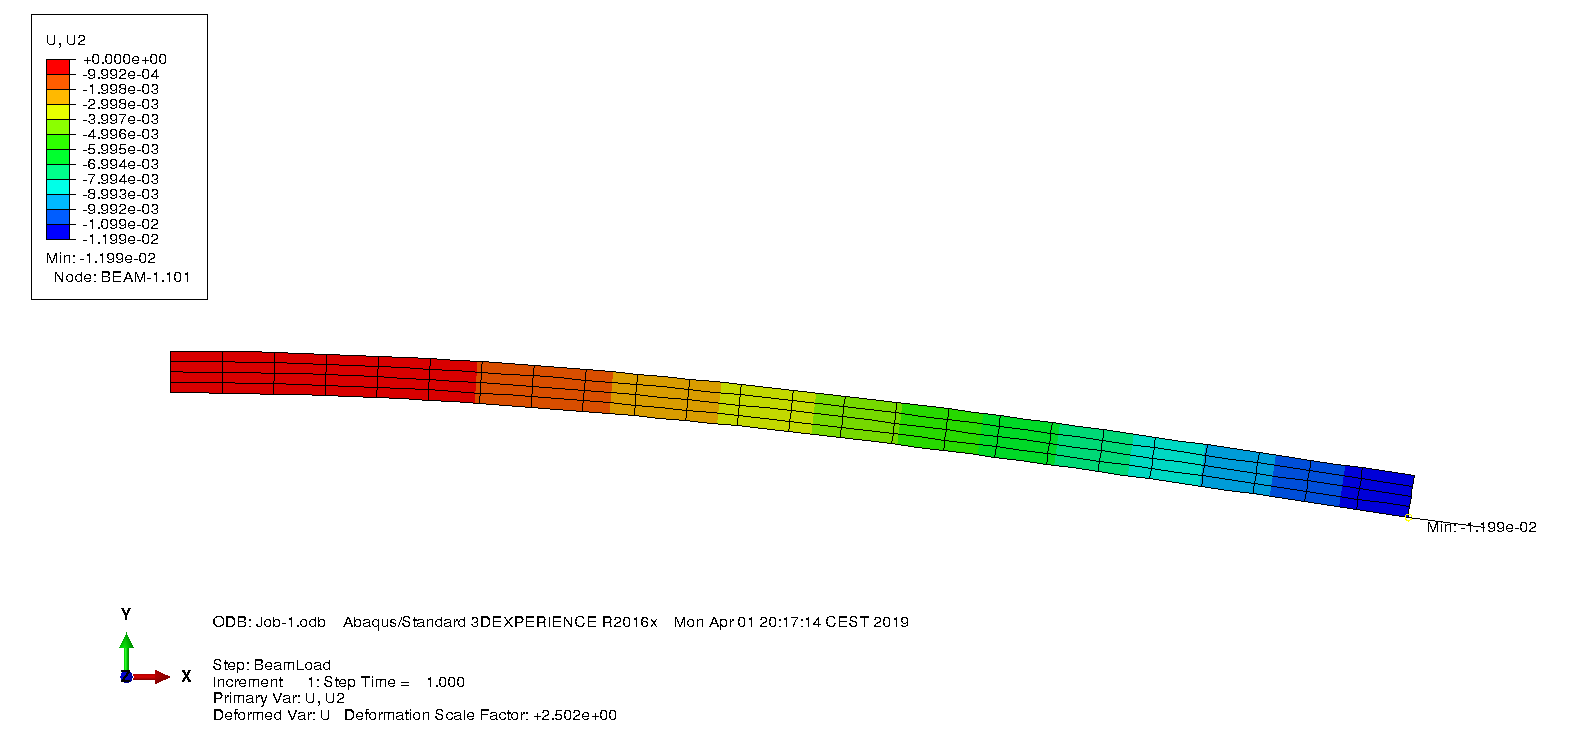
\includegraphics[width=0.8\textwidth]{pics/4_24_CPS8}
  \caption{maximal displacment: -11.99 mm}
\end{figure}
\FloatBarrier
\pagebreak
\subsubsection{CPS4R}
\begin{figure}[!htb]
  \centering
  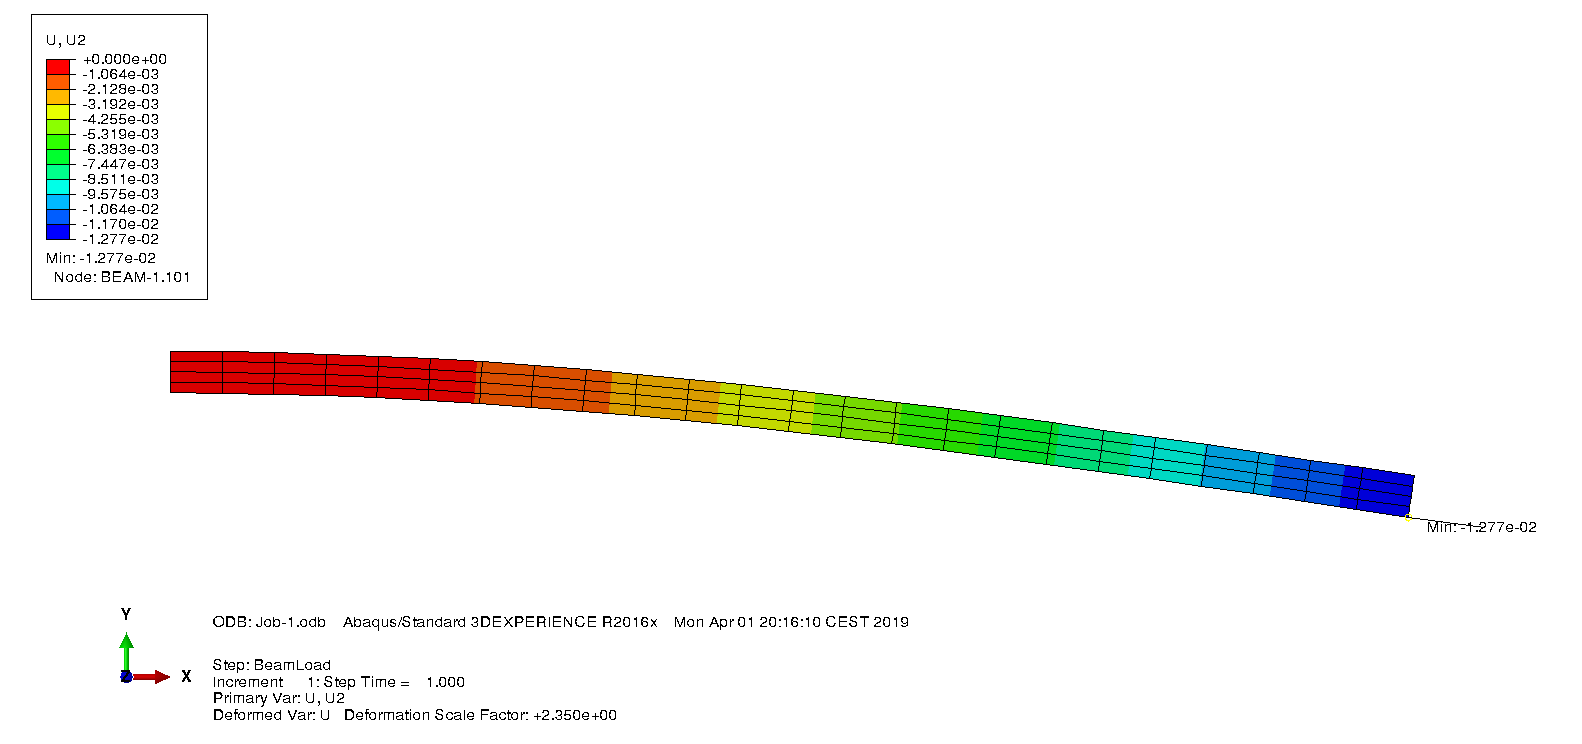
\includegraphics[width=0.8\textwidth]{pics/4_24_CPS4R}
  \caption{maximal displacment: -12.77 mm}
\end{figure}
\FloatBarrier
\subsubsection{CPS8R}
\begin{figure}[!htb]
  \centering
  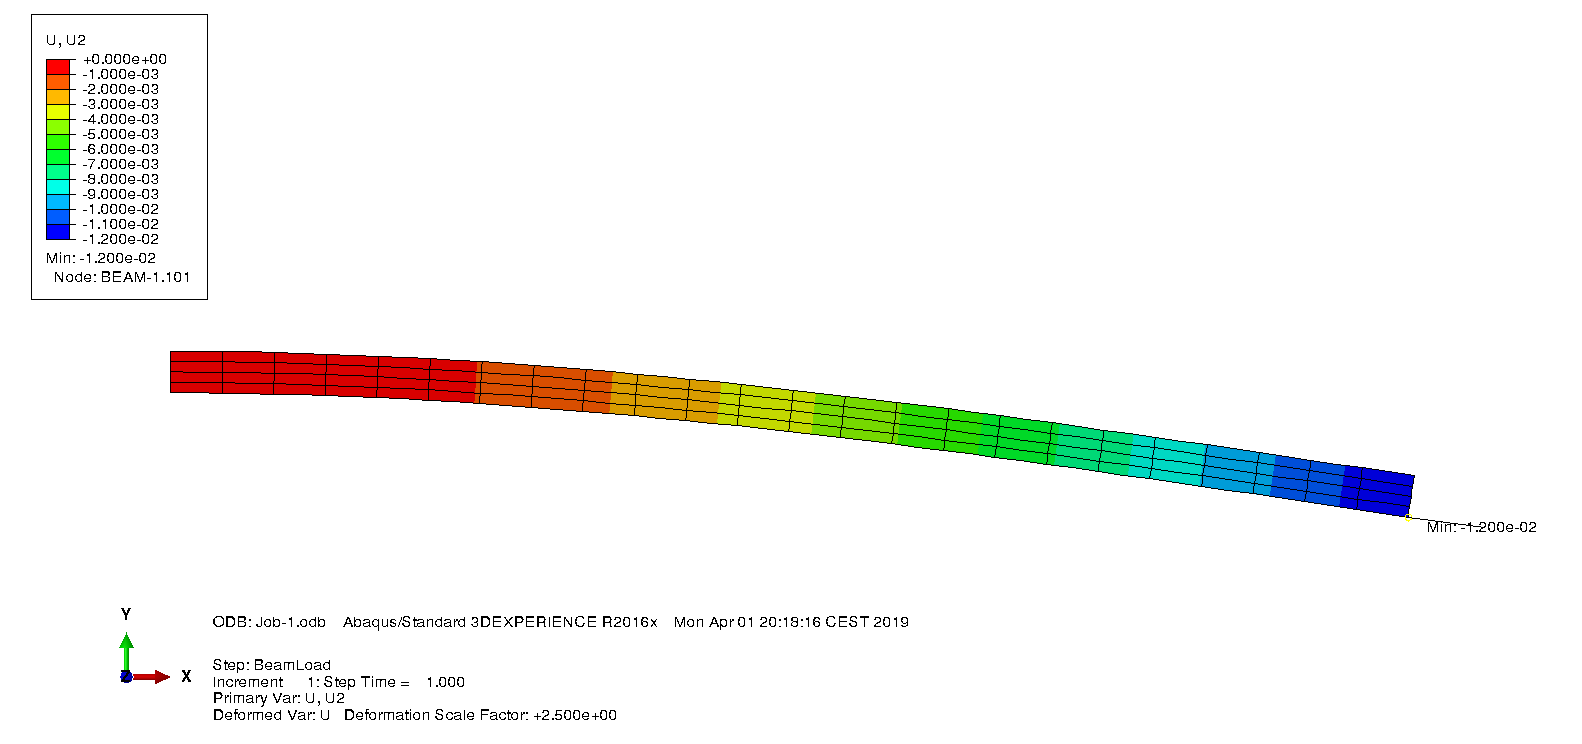
\includegraphics[width=0.8\textwidth]{pics/4_24_CPS8R}
  \caption{maximal displacment: -12.00 mm}
\end{figure}
\FloatBarrier
\pagebreak
\section{Disscussion}
The Discussion refers to the questions in the assignment.
\begin{quote}
How do the numerical results change with respect to the analytical
one? Which mesh \& element configuration's is/are closest to the
analytical solution? Conversely, which one's is/are farthest from it?
\end{quote}
The closest solution calculated to the analytical result can be 
achieved with an appropriate mesh size (4 x 24).  Also, the correct 
numerical method can have a positive impact with a lower mesh size (2 x 12). 
Overall, using low mesh size and linear methods gives the most inaccurate solutions.
\begin{quote}
How does changing the number of elements influence the results
(2x12 vs. 4x24 elms)?
How does changing the element type influence the results? (CPS4
vs. CPS8)?
\end{quote}
A higher number of elements gives us, in general, more accurate solutions. However, 
using more nodes also results in more accuracy.
\begin{quote}
How does changing 
the integration method 
influence the results
(CPS4 vs. CPS4R; CPS8 vs. CPS8R)?
\end{quote}
Reducing the integration method is only effective with enough number of elements. 
Reducing with a low number of elements will give us inaccurate solutions, as the 
model will then be "too" reduced.
\begin{quote}
Give brief explanations on why the results change with respect to
different mesh \& element configurations using the terminologies
explained during the course (i.e. hourglassing, shear locking)?
\end{quote}
Inaccurate solutions are caused by the shear looking effect. With a 
small element size as 2 x 12, and also with further reducing the edges 
will then not be able to bend and deform, ending in shearing. The 
desired effect on our beam should be bending.

The hourglassing effect comes up if we apply the reduced integration 
method on also low element mesh size on our part, with a higher 
displacement in the result. The elements are too flexible, as 
the element matrix has insufficient stiffness.
\end{document}